\documentclass[12pt; a4paper]{book}
\usepackage{graphicx} %for pic
\usepackage[utf8x]{inputenc}
\usepackage[russian]{babel} % for rus

\usepackage{fancyhdr}  % for beauty hat, floor and sides style
\pagestyle{fancy}

\usepackage{xcolor}  % for href and href colour
\usepackage{hyperref}

\usepackage{amsmath} 

\begin{document} 

\frontmatter
\title{Технологии программирования\\ 2 семестр}
\author{Автор} 
\date{Весна 2020}
\maketitle
Это конспект лекций читаемых в МФТИ Старичковым Н.. Название курса "Технологическое Программирование", 
\tableofcontents

\mainmatter
%\fancyhead[L] {Проектирование ПО}
\chapter{Проектирование ПО}

\section{Этапы проектирования. (1я часть)}
\begin{enumerate}
\item Формирование требований
\item Разработка концепции
\item Техническое задание
\item Экскизный проект
\item Технический проект
\item Разработка документации
\item Поставка / ввод в действие
\item Сопровождение
\end{enumerate}\

\subsection{Формирование требований}
\begin{enumerate}
\item Общение с клиентом
\item Общение с пользователем
\item Анализ прикладной части
\item Формирование оценок требуемой производительности
\item Обоснование объекта
\item Исследование необходимости проекта (какие проблемы решает).
\item Формирование требований пользователя
\item[-] \textbf{подготовка отчета по этапу}
\end{enumerate}

\subsection{Разработка концепции}
\begin{enumerate}
\item Изучение объекта автоматизации
\item Проведение необходимых НИР (научно исследовательских работ)
\item Разработка вариантов концепции
\item Выбор формата (это веб ресурс / приложение)
\item Целевое оборудование
\item Построение высокоуровневой архитектуры системы
\item Выбор / Разработка новых алгоритмов / технологий
\item[-] \textbf{подготовка отчета по этапу}
\end{enumerate}

\subsection{Техническое задание}
Основное отличие от документации в том что тут находятся данные о требованиях
предоставляемых разработчику (например должно работать с 90\% железа), которые пользователь может не видеть. А документация как раз доступна для пользователя.
\begin{enumerate}
\item Описание системы
\item Описание функциональности
\item \hangindent=6cm \hangafter=2 \noindent Описание сценариев использования\\ {\footnotesize Например, пользователь обычно либо только выгружает видео или только стримит, и ему не нужно выделять ресурсов для одновременности этих процессов.}
\item Условия сдачи
\end{enumerate}

\subsection{Эскизный проект}
\begin{enumerate}
\item Разработка прототипов частей системы
\item Оценка производительности и качества
\item Изменение прототипов
\item[-] Часто это MVP (minimal viable product)
\item[-] Иногда это система с базовой функциональностью
\item[-] Иногда с урезанным проектом
\item[-] Иногда менее производительная
\item[-] \textbf{подготовка отчета по этапу}
\end{enumerate}
\subsection{Технический проект}
\begin{enumerate}
\item Разработка частей системы
\item Разработка документации
\item  Разработка заданий на проектирование и реализацию основных частей
\item Тестирование
\item Оценка качеств и производительности
\end{enumerate}

\subsection{Рабочая документация}
\begin{enumerate}
\item Сценарии использования
\item Описание логики работы
\item Описание производительности
\item Примеры использования
\item Обучающие мероприятия
\end{enumerate}

\subsection{Ввод в действие}
\begin{enumerate}
\item Подготовка объекта автоматизации
\item Подготоввка персонала
\item Комплектация системы поставляемыми изделиями
\item Проведение предварительных испытаний
\item Опытная эксплуатация
\item Приемочные испытания
\end{enumerate}

\subsection{Сопровождение системы}
\begin{enumerate}
\item Гарантийные обязательства
\item Послегарантийное обслуживание
\end{enumerate}
\newpage

\section{UML}
Проектирование ПО (2я часть). 
\subsection{Диаграмма вариантов использования}
\begin{figure}[!hbp]
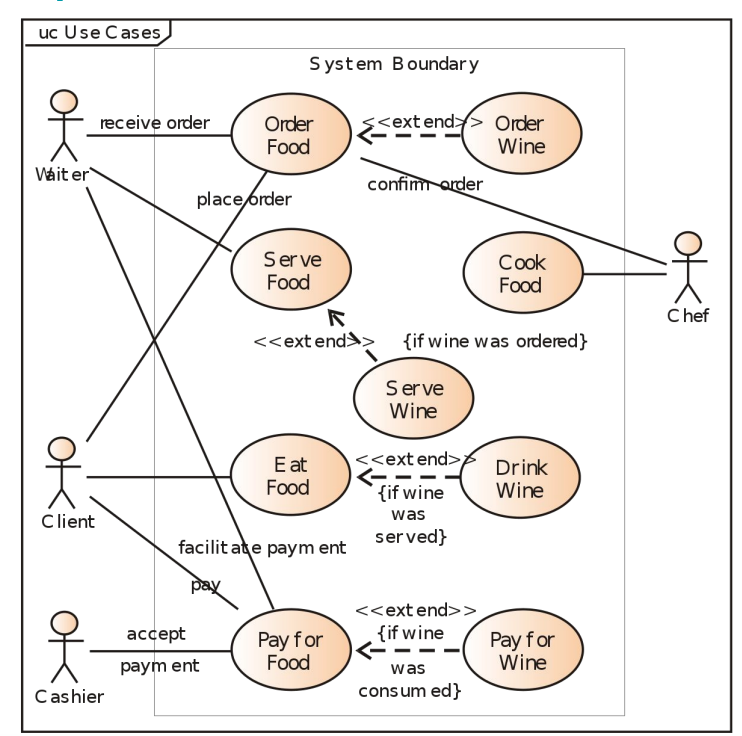
\includegraphics[angle=0, width=\textwidth]{IMG/1} 
\end{figure}
\newpage

\subsection{Диаграмма классов}
\begin{figure}[!hbp]
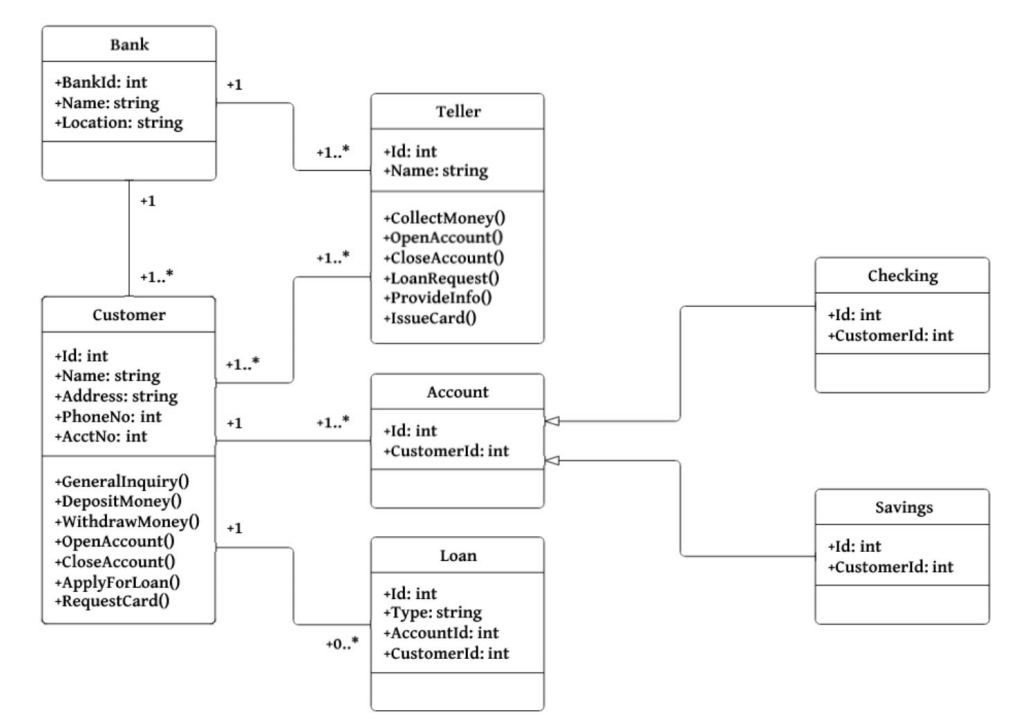
\includegraphics[angle=0, width=\textwidth]{IMG/2} \\
\end{figure}
Есть разные связи: 
\begin{enumerate}
\item[1] (Например король Артур и его лошадь) когда один объект так же перестает существовать
\item[1-1] Лошадь и всадник, когда они существуют по отдельности
\end{enumerate}
Так, например, в базе данных при удалении одного элемента, элементы, связанные с ним связью "1" так же будут не действительны.
\newpage

\subsection{Диаграмма последовательности}
\begin{figure}[!hbp]
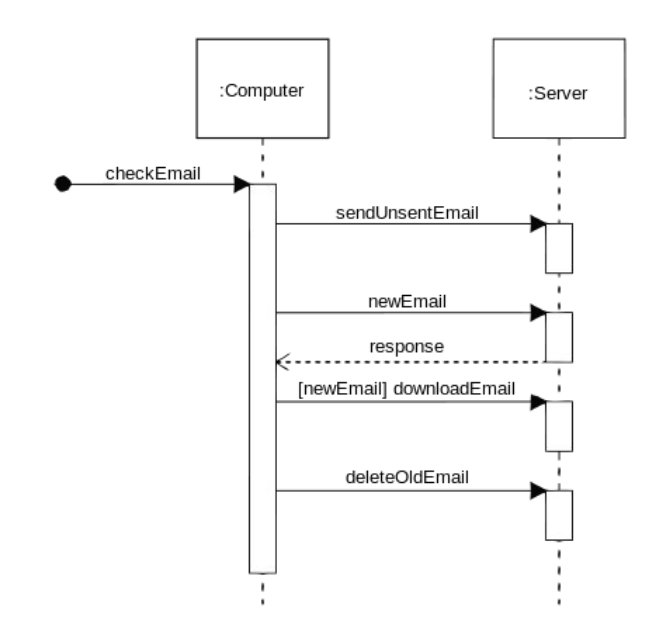
\includegraphics[angle=0, width=0.8\textwidth]{IMG/3} \\
\end{figure}
Рассмотрим на примере заселения.  В процессе участвуют Мы, Олег (поселяющий), Врач, кастелянша, деканат
Сначала мы идем к камендантше, затем идем к Олегу, он дает "a prove".  После идем к врачу, потом уже  к кастелянше.\\
Причем подключаются блоки в разных случаях: Сказал ли Олег Да или Нет? (Блок договориться с Олегом)\\
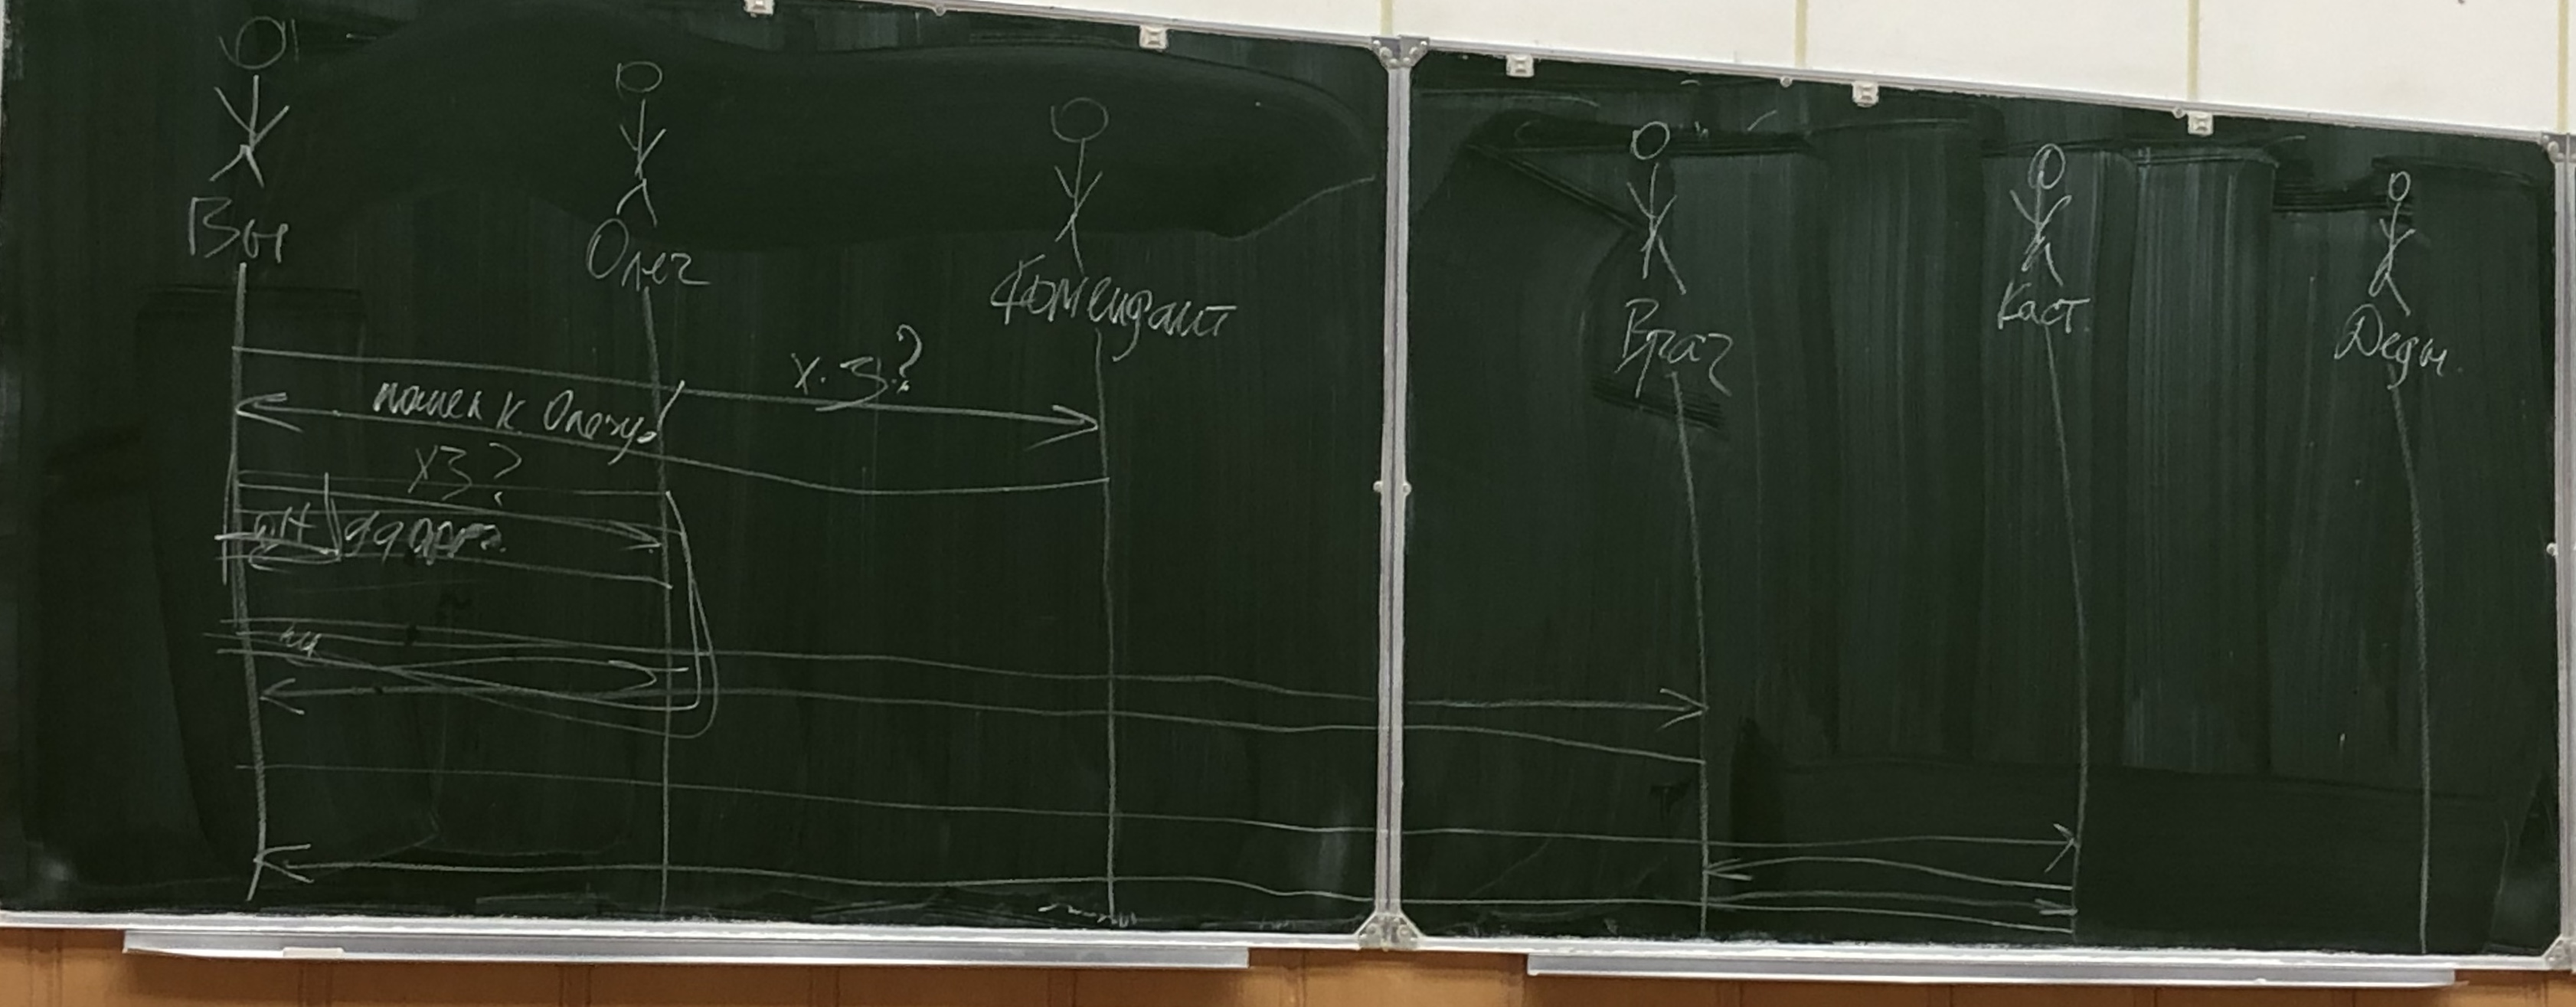
\includegraphics[angle=0, width=\textwidth]{IMG/IMG_0818.jpg} \\
\newpage

\subsection{Диаграмма состояний}
\begin{figure}[!htbp]
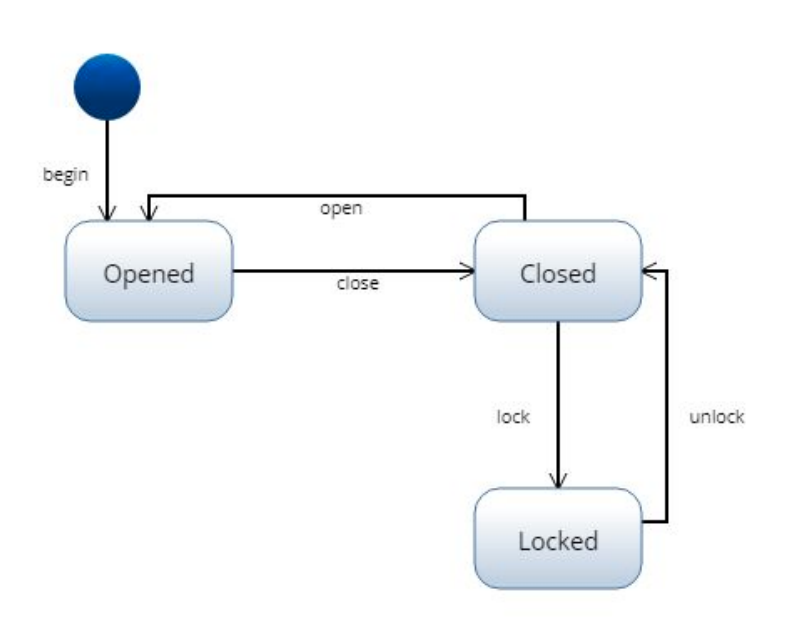
\includegraphics[angle=0, width=\textwidth]{IMG/4} \\
\end{figure}
\begin{figure}[!htbp]
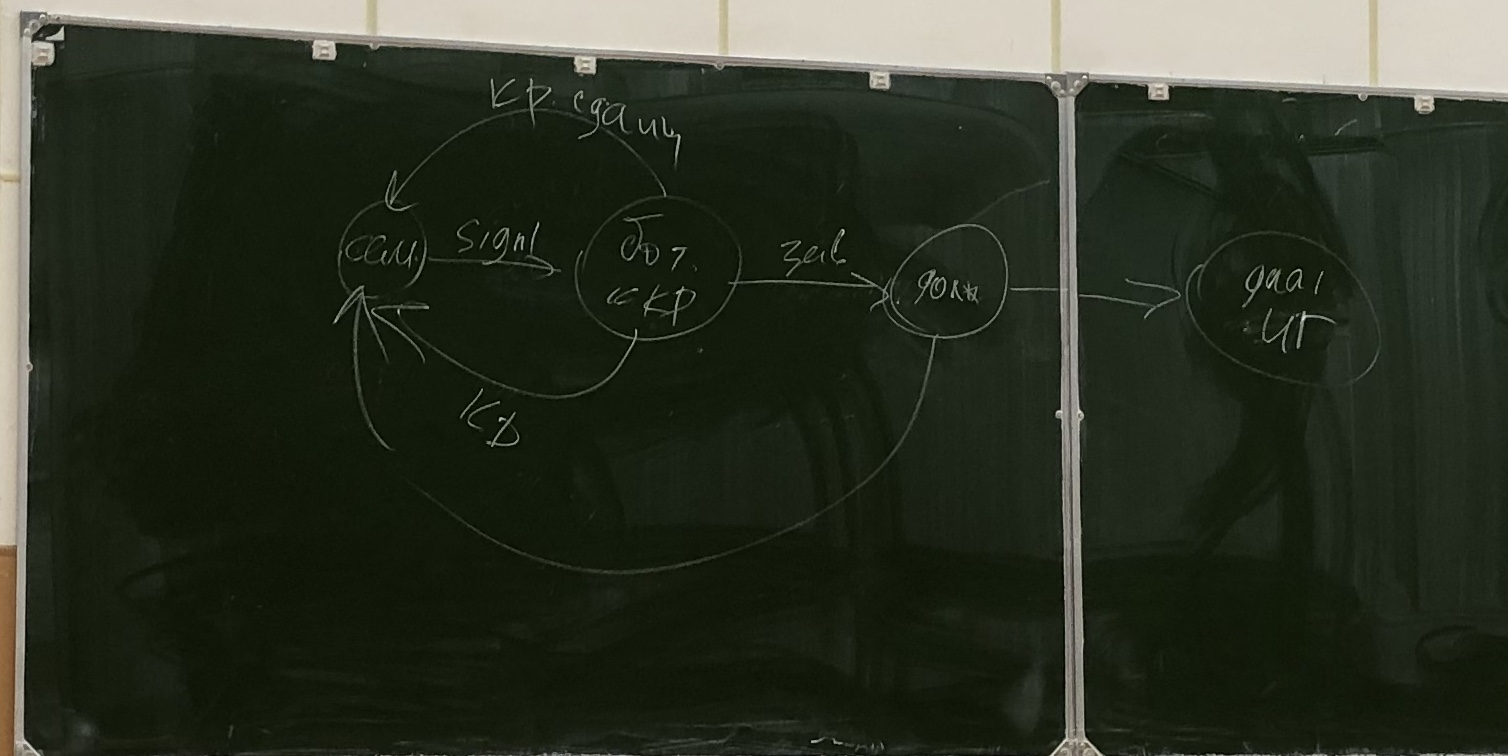
\includegraphics[angle=0, width=\textwidth]{IMG/IMG_0820.jpg} \\
\end{figure}
Диаграмма для студента:
Студент находится в состоянии "учусь", иногда переходит к состоянию "ботаю кр", дальше если кр не сдана то к состоянию "должник" и так далее...\\

Так с экраном. Если вы нажимаете Esc проваливаетесь на рабочий стол, дальше если открываете приложение проваливаетесь еще куда-то и т. д. \\
Еще когда мы открываем на телефоне карточки для платежа, яркость телефона выкручивается на максимум. Иногда телефон забывает вернуть яркость обратно, И ОН ВЫЖИГАЕТ ГЛАЗА) И нужно прописывать при переходе это.
\newpage

\subsection{Диаграма деятельности}
\begin{figure}[!htbp]
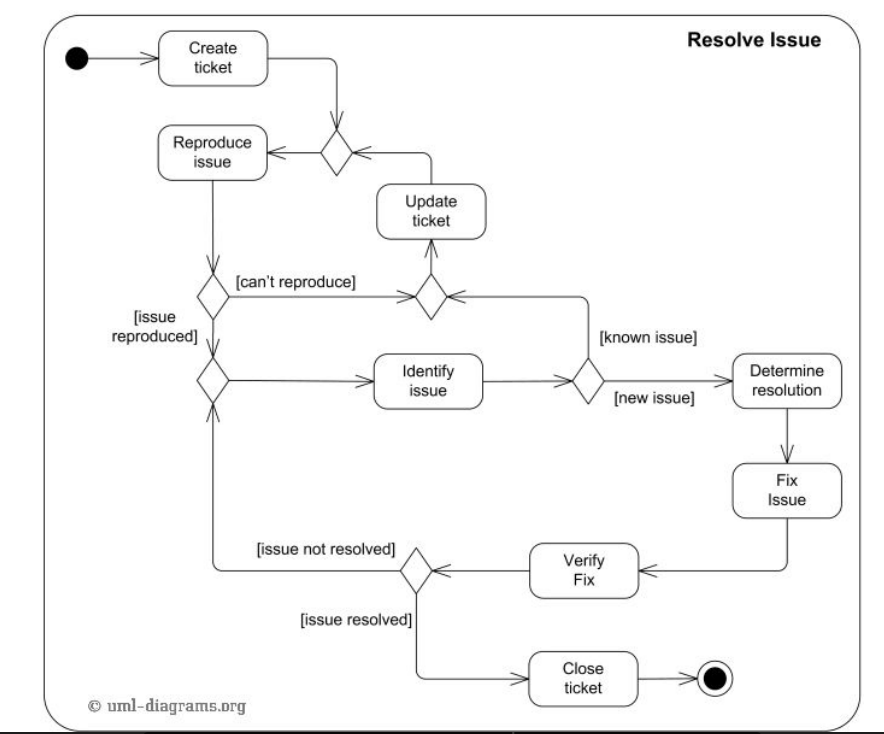
\includegraphics[angle=0, width=\textwidth]{IMG/5} \\
\end{figure}

Описание порядка набора действий на формальном языке с указанием что кто вызывает, по которой можно все восстановить. \\
\begin{figure}[!htbp]
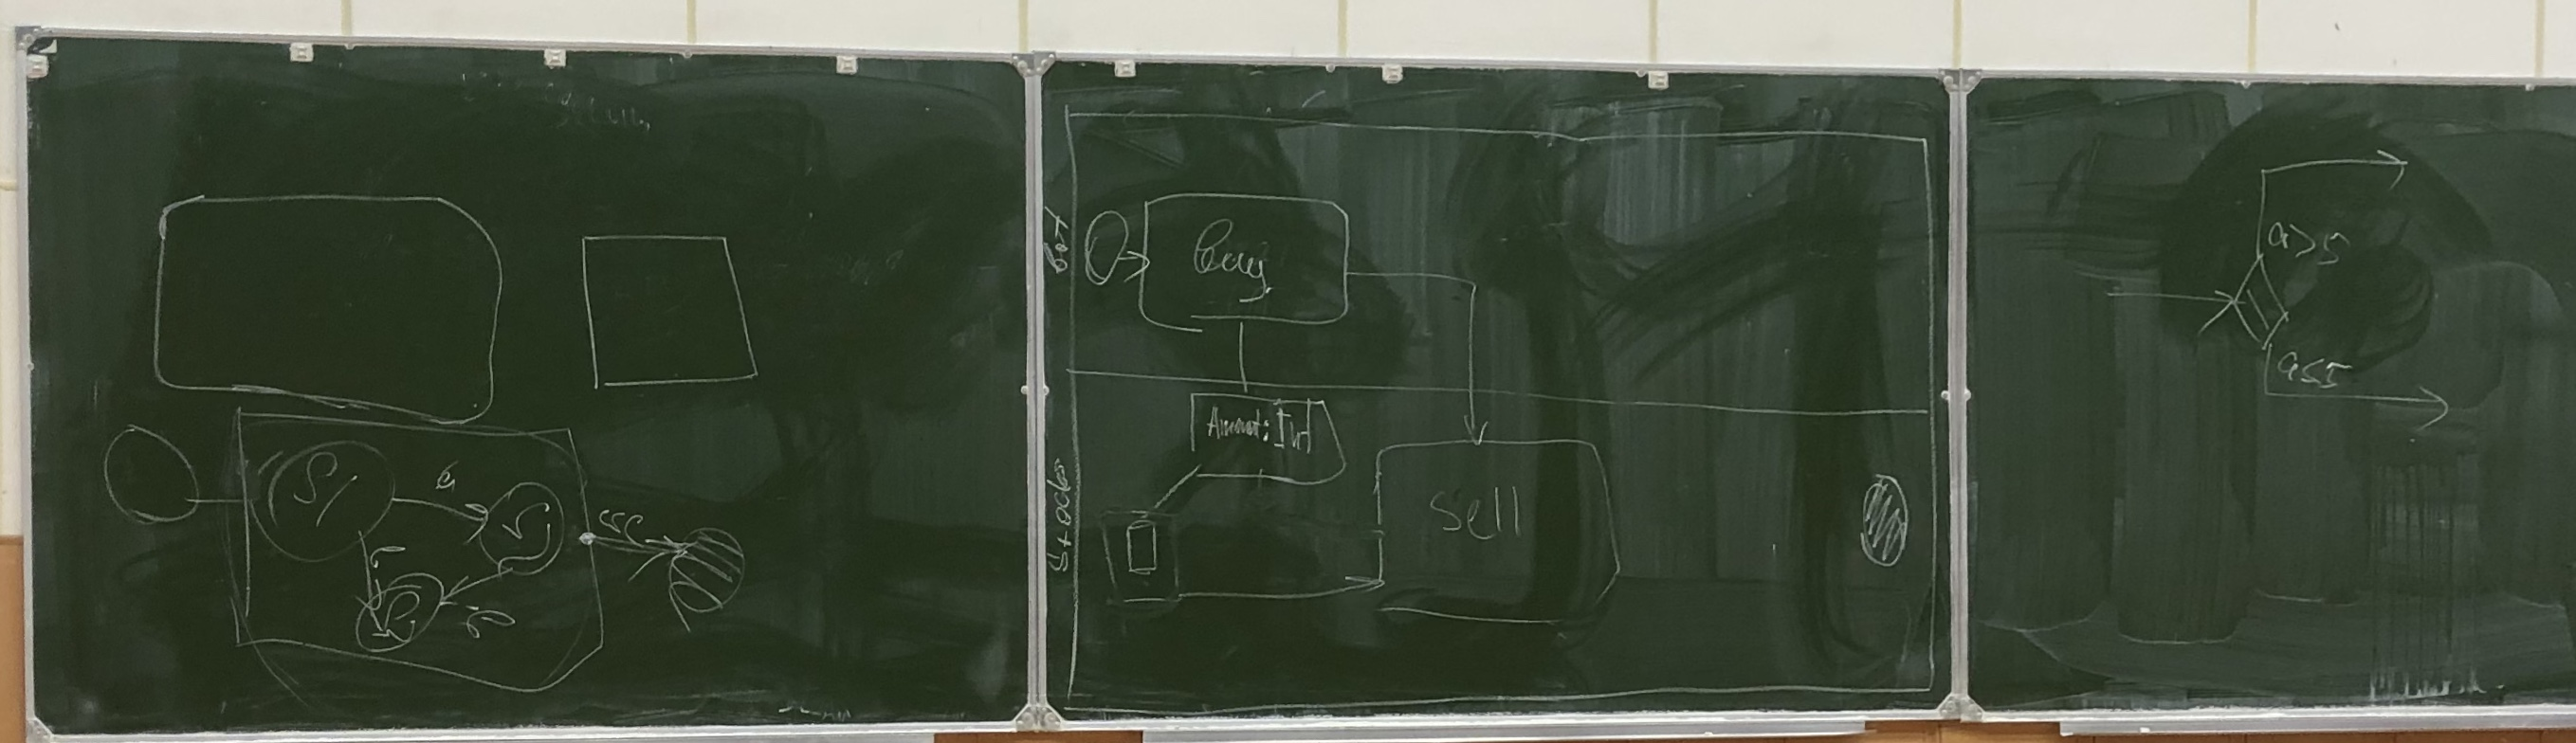
\includegraphics[angle=0, width=\textwidth]{IMG/IMG_0823.jpg} \\
\end{figure}

\#операция - с закругленными, объект - прямоугольник с острыми углами \\
например у bot 'а операция buy передает объект "ammount int" в операцию биржи(snoks) выполняя ее\\
\#терминальное состояние -- состояние конца операции для которой рисуется диаграмма \\
Еще есть условия (Например Ammount > 5/ <5...) \\
\#условия рисуются ромбиком\\\

\begin{figure}[!htbp]
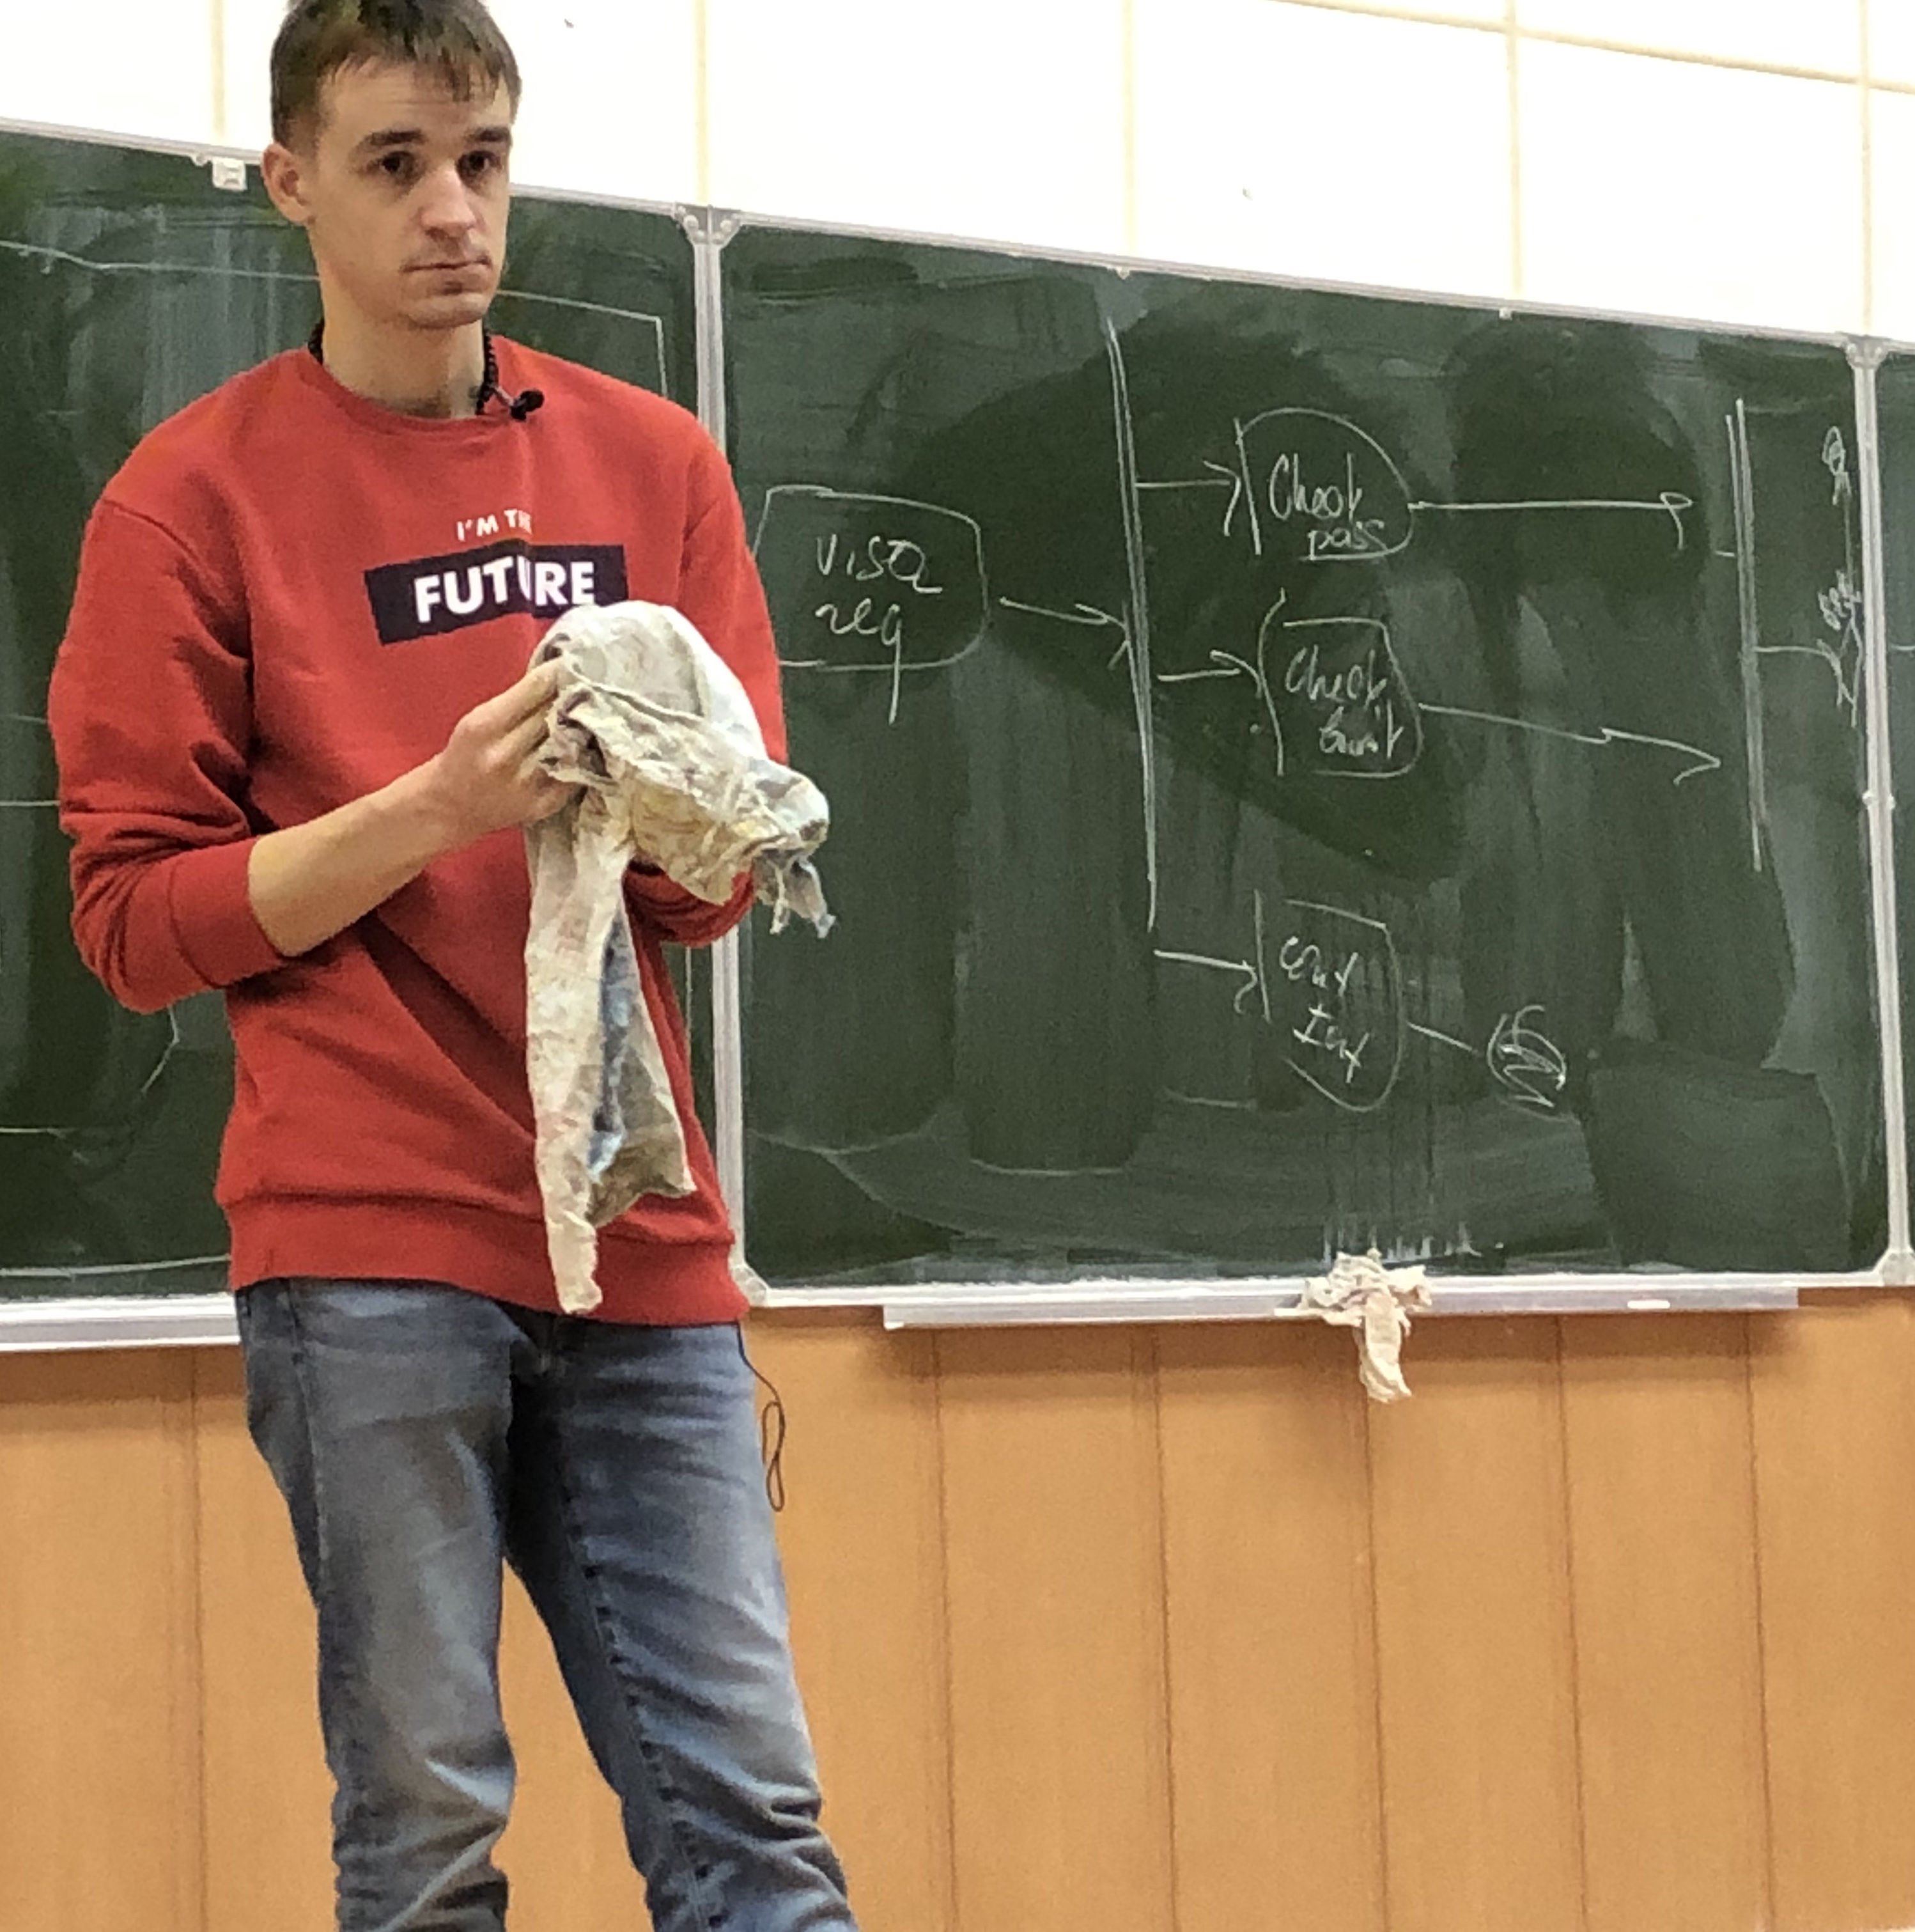
\includegraphics[angle=0, width=\textwidth]{IMG/IMG_0826.jpg} \\
\end{figure}

Еще есть распаралеливание и при завершении одного потока завершается только один поток. Потоки можно сливать. 
Например я хочу получить визу. Система паралельнор проверяет паспорт, проверяет банковский счет, и последняя, сразу завершаемая: передать в интерпол что поступил запрос. Дальше все сливается и виза дается/или нет.\\
\newpage

\end{document}


\subsection{}
\begin{enumerate}
\item 
\item 
\item 
\item 
\item 
\item 
\item \end{enumerate}
\textbf{} %make bold
\hangindent=6cm \hangafter=2 \noindent % 1st - indent length, 2nd - numb of str without indent

\definecolor{linkcolor}{HTML}{799B03} % цвет ссылок
\definecolor{urlcolor}{HTML}{799B03} % цвет гиперссылок
 
\hypersetup{linkcolor=linkcolor,urlcolor=urlcolor, colorlinks=true}

%%%%%%%%%%%%%%%%%%%%%%
Редакторы:  \href{https://vk.com/akira33333}{Фреик Александр} \href{https://github.com/Falier77777}{git}\\

\begin{titlepage}
\begin{center}
\large\textbf{Московский Физико-Технический Институт}\\
\large\textbf{(государственный университет)}
\vfill
\line(1,0){350}\\[2mm]
\huge\textbf{Технологии программирования\\ 2 семестр, 2020 год}\\
\line(1,0){350}\\[2mm]
\vfill
\line(1,0){350}\\[1mm]
{\normalsize Лектор: Старичков Никита\\\
Редакторы:  \href{https://vk.com/akira33333}{Фреик Александр} \href{https://github.com/Falier77777}{git}}\\
\large ФПМИ\\
\line(1,0){350}\\[1mm]
\end{center}
\end{titlepage}
%%%%%%%%%%%%%%%%%%%%%%%
